\documentclass[]{article}
\usepackage{lmodern}
\usepackage{amssymb,amsmath}
\usepackage{ifxetex,ifluatex}
\usepackage{fixltx2e} % provides \textsubscript
\ifnum 0\ifxetex 1\fi\ifluatex 1\fi=0 % if pdftex
  \usepackage[T1]{fontenc}
  \usepackage[utf8]{inputenc}
\else % if luatex or xelatex
  \ifxetex
    \usepackage{mathspec}
  \else
    \usepackage{fontspec}
  \fi
  \defaultfontfeatures{Ligatures=TeX,Scale=MatchLowercase}
\fi
% use upquote if available, for straight quotes in verbatim environments
\IfFileExists{upquote.sty}{\usepackage{upquote}}{}
% use microtype if available
\IfFileExists{microtype.sty}{%
\usepackage{microtype}
\UseMicrotypeSet[protrusion]{basicmath} % disable protrusion for tt fonts
}{}
\usepackage[margin=1in]{geometry}
\usepackage{hyperref}
\hypersetup{unicode=true,
            pdftitle={Exerciții de seminar 2},
            pdfborder={0 0 0},
            breaklinks=true}
\urlstyle{same}  % don't use monospace font for urls
\usepackage{natbib}
\bibliographystyle{plainnat}
\usepackage{graphicx,grffile}
\makeatletter
\def\maxwidth{\ifdim\Gin@nat@width>\linewidth\linewidth\else\Gin@nat@width\fi}
\def\maxheight{\ifdim\Gin@nat@height>\textheight\textheight\else\Gin@nat@height\fi}
\makeatother
% Scale images if necessary, so that they will not overflow the page
% margins by default, and it is still possible to overwrite the defaults
% using explicit options in \includegraphics[width, height, ...]{}
\setkeys{Gin}{width=\maxwidth,height=\maxheight,keepaspectratio}
\IfFileExists{parskip.sty}{%
\usepackage{parskip}
}{% else
\setlength{\parindent}{0pt}
\setlength{\parskip}{6pt plus 2pt minus 1pt}
}
\setlength{\emergencystretch}{3em}  % prevent overfull lines
\providecommand{\tightlist}{%
  \setlength{\itemsep}{0pt}\setlength{\parskip}{0pt}}
\setcounter{secnumdepth}{5}
% Redefines (sub)paragraphs to behave more like sections
\ifx\paragraph\undefined\else
\let\oldparagraph\paragraph
\renewcommand{\paragraph}[1]{\oldparagraph{#1}\mbox{}}
\fi
\ifx\subparagraph\undefined\else
\let\oldsubparagraph\subparagraph
\renewcommand{\subparagraph}[1]{\oldsubparagraph{#1}\mbox{}}
\fi

%%% Use protect on footnotes to avoid problems with footnotes in titles
\let\rmarkdownfootnote\footnote%
\def\footnote{\protect\rmarkdownfootnote}

%%% Change title format to be more compact
\usepackage{titling}

% Create subtitle command for use in maketitle
\newcommand{\subtitle}[1]{
  \posttitle{
    \begin{center}\large#1\end{center}
    }
}

\setlength{\droptitle}{-2em}
  \title{Exerciții de seminar 2}
  \pretitle{\vspace{\droptitle}\centering\huge}
  \posttitle{\par}
\subtitle{Regresie}
  \author{}
  \preauthor{}\postauthor{}
  \date{}
  \predate{}\postdate{}

\usepackage{booktabs}
\usepackage{longtable}
\usepackage{framed,color}
\definecolor{shadecolor}{RGB}{248, 248, 248}
%\definecolor{shadecolor1}{RGB}{216,225,235}
%\definecolor{framecolor}{RGB}{108,123,13}

%\definecolor{shadecolor}{RGB}{226, 255, 241}
\definecolor{shadecolor1}{RGB}{217,225,199}
\definecolor{framecolor}{RGB}{60,179,113}

\ifxetex
  \usepackage{letltxmacro}
  \setlength{\XeTeXLinkMargin}{1pt}
  \LetLtxMacro\SavedIncludeGraphics\includegraphics
  \def\includegraphics#1#{% #1 catches optional stuff (star/opt. arg.)
    \IncludeGraphicsAux{#1}%
  }%
  \newcommand*{\IncludeGraphicsAux}[2]{%
    \XeTeXLinkBox{%
      \SavedIncludeGraphics#1{#2}%
    }%
  }%
\fi

\newenvironment{frshaded*}{%
  \def\FrameCommand{\fboxrule=\FrameRule\fboxsep=\FrameSep \fcolorbox{framecolor}{shadecolor1}}%
  \MakeFramed {\advance\hsize-\width \FrameRestore}}%
{\endMakeFramed}

\newenvironment{rmdblock}[1]
  {\begin{frshaded*}
  \begin{itemize}
  \renewcommand{\labelitemi}{
    \raisebox{-.7\height}[0pt][0pt]{
      {\setkeys{Gin}{width=2em,keepaspectratio}\includegraphics{images/icons/#1}}
    }
  }
  \item
  }
  {
  \end{itemize}
  \end{frshaded*}
  }

\newenvironment{rmdcaution}
  {\begin{rmdblock}{caution}}
  {\end{rmdblock}}
% \newenvironment{rmdinsight}
%   {\begin{rmdblock}{insight}}
%   {\end{rmdblock}}
\newenvironment{rmdexercise}
  {\begin{rmdblock}{exercise}}
  {\end{rmdblock}}
\newenvironment{rmdtip}
  {\begin{rmdblock}{tip}}
  {\end{rmdblock}}


%%%%%%%%%%%%%%%%%%%%%%%%%%%%%%%%%%%%%%%%%%%%%%%%%%%%%%%%%%%%%%%%%%%%%%%%%%%%%%%%%%%%%%%%%%%%%%%%%%%%%%%%%%%%%%%%%%%%%
%%%%%%%%%%% For insight block %%%%%%%%%%%%%%%%%%%%%%%%%%
\definecolor{shadecolor_insight}{RGB}{223,240,216}
\definecolor{framecolor_insight}{RGB}{136,193,137}

%\definecolor{shadecolor_insight}{RGB}{217,225,199}
%\definecolor{framecolor_insight}{RGB}{60,179,113}

\newenvironment{frshaded_insight*}{%
  \def\FrameCommand{\fboxrule=\FrameRule\fboxsep=\FrameSep \fcolorbox{framecolor_insight}{shadecolor_insight}}%
  \MakeFramed {\advance\hsize-\width \FrameRestore}}%
{\endMakeFramed}

\newenvironment{rmdblock_insight}[1]
  {\begin{frshaded_insight*}
  \begin{itemize}
  \renewcommand{\labelitemi}{
    \raisebox{-.7\height}[0pt][0pt]{
      {\setkeys{Gin}{width=2em,keepaspectratio}\includegraphics{images/icons/#1}}
    }
  }
  \item
  }
  {
  \end{itemize}
  \end{frshaded_insight*}
  }

\newenvironment{rmdinsight}
  {\begin{rmdblock_insight}{insight}}
  {\end{rmdblock_insight}}

%%%%%%%%%%%%%%%%%%%%%%%%%%%%%%%%%%%%%%%%%%%%%%%%%%%%%%%%%%%%%%%%%%%%%%%%%%%%%%%%%%%%%%%%%%%%%%%%%%%%%%%%%%%%%%%%%%%%%
\usepackage{subfigure}
\usepackage{booktabs}
\usepackage{slashbox}
\usepackage{color}
%%%%%%%%%%%%%%%%%%%%%%%%%%%%%%%%%%%%%%%%%
\definecolor{linkcol}{rgb}{0,0,0.4}
\definecolor{citecol}{rgb}{0.5,0,0}

% Change this to change the informations included in the pdf file
% \usepackage[pagebackref]{hyperref}
% \usepackage[verbose]{backref}
\usepackage[hyperpageref]{backref}
% \backrefsetup{verbose=false}
% \PassOptionsToPackage{pagebackref}{hyperref}
% See hyperref documentation for information on those parameters

\hypersetup
{
bookmarksopen=true,
pdftitle="Curs Instrumente Statistice pentru Finante",
pdfauthor="Alexandru Amarioarei",
pdfsubject="Laboratoare Instrumente Statistice pentru Finante", %subject of the document
pdfmenubar=true, %menubar shown
pdfhighlight=/O, %effect of clicking on a link
colorlinks=true, %couleurs sur les liens hypertextes
pdfpagemode=None, %aucun mode de page
pdfpagelayout=SinglePage, %ouverture en simple page
pdffitwindow=true, %pages ouvertes entierement dans toute la fenetre
linkcolor=linkcol, %couleur des liens hypertextes internes
citecolor=citecol, %couleur des liens pour les citations
urlcolor=linkcol %couleur des liens pour les url
}


% set the back references
\renewcommand*{\backref}[1]{}
\renewcommand*{\backreftwosep}{ și~} % inserted between entries 
                              % in a list of two entries, 
                              % default is " and~".
\renewcommand*{\backreflastsep}{ și~} % inserted between the last 
                               % two entries of a list with more
                               % than two entries, default is ", and~".
\renewcommand*{\backrefalt}[4]{%
    \ifcase #1 (Necitat.)%
    \or        (Citat la pagina~#2.)%
    \else      (Citat la paginile~#2.)%
    \fi}

%%%%%%%%%%%%%%%%%%%%%%%%%%%%%%%%%%%%%%%%%%%%%%%%%%%%%%%%%%%%%%%%%%%%%%%%%%%%%%%%%%%%%%%%%%%%%%%%%%%%%%%%%%%%%%%%%%%%%
%CITEVA DEFINITII
\def\om{\omega}
\def\Om{\Omega}
\def\et{\eta}
\def\td{\tilde{\delta}}
\def\m{{\mu}}
\def\n{{\nu}}
\def\k{{\kappa}}
\def\l{{\lambda}}
\def\L{{\Lambda}}
\def\g{{\gamma}}
\def\a{{\alpha}}
\def\e{{\varepsilon}}
\def\b{{\beta}}
\def\G{{\Gamma}}
\def\d{{\delta}}
\def\D{{\Delta}}
\def\t{{\theta}}
\def\s{{\sigma}}
\def\S{{\Sigma}}
\def\z{{\zeta}}
\def\qed{\hfill\Box}
\def\ds{\displaystyle}
\def\mc{\mathcal}
%%%%%%%%%%%%%%%%%%%%%%%%%%%%%%%%%%%%%%%%%%%%%%%%%%%%%%%%%%%%%%%%%%%%%%%%%%%%%%%%%%%%%%%%%%%%%%%%%%%%%%%%%%%%%%%%%%%%%%
\def\1{{\mathbf 1}}
\def\CC{{\mathbb C}}
\def\VV{{\mathbb V}}
\def\RR{{\mathbb R}}
\def\QQ{{\mathbb Q}}
\def\ZZ{{\mathbb Z}}
\def\PP{{\mathbb P}}
\def\EE{{\mathbb E}}
\def\NN{{\mathbb N}}
\def\FF{{\mathbb F}}
%\def\SS{{\mathbb S}}
\def\MA{{\mathcal A}}
\def\MO{{\mathcal O}}
\def\MF{{\mathcal F}}
\def\ME{{\mathcal E}}
\def\MR{{\mathcal R}}
\def\MB{{\mathcal B}}
\def\MM{{\mathcal M}}
\def\MN{{\mathcal N}}
\def\MU{{\mathcal U}}
\def\MP{{\mathcal P}}
\def\MS{{\mathcal S}}
\def\MBS{{\mathbf S}}
\def\MX{{\bm{ \mathscr X}}}

% independent sign
\newcommand\independent{\protect\mathpalette{\protect\independenT}{\perp}}
\def\independenT#1#2{\mathrel{\rlap{$#1#2$}\mkern2mu{#1#2}}}

\renewcommand\tablename{Tab.}
\renewcommand{\figurename}{Fig.}
\renewcommand\refname{Referințe}

%%%%%%%%%%%%%%%%%%%%%%%%%%%%%%%%%%%%%%%%%%%%%%%%%%%%%%%%%%%%%%%%%%%%%%%%%%%%%%%%%%%%%%%%%%%%%%%%%%%%%%%%%%%%%%%%%%%%%
%Header and Footer
\usepackage{fancyhdr}

\pagestyle{fancy}
\fancyhf{}
\rhead{Universitatea din Bucure\c sti\\ Facultatea de Matematic\u a \c si Informatic\u a}
\lhead{\textit{Curs}: Instrumente Statistice pentru Finan\c te\\ \textit{Instructor}: A. Am\u arioarei}
\rfoot{Pagina \thepage}
\lfoot{Grupa: 403}
%%%%%%%%%%%%%%%%%%%%%%%%%%%%%%%%%%%%%%%
\usepackage{booktabs}
\usepackage{longtable}
\usepackage{array}
\usepackage{multirow}
\usepackage[table]{xcolor}
\usepackage{wrapfig}
\usepackage{float}
\usepackage{colortbl}
\usepackage{pdflscape}
\usepackage{tabu}
\usepackage{threeparttable}
\usepackage{threeparttablex}
\usepackage[normalem]{ulem}
\usepackage{makecell}

\begin{document}
\maketitle

%%%%%%%%%%%%%%%%%%%%%%%%
\thispagestyle{fancy}

Obiectivul acestui seminar este de a prezenta câteva exerciții de
regresie liniară.

\section{Regresie liniară simplă}\label{regresie-liniara-simpla}

\subsection{Interpretări geometrice}\label{interpretari-geometrice}

În această secțiune încercăm să abordăm problema de regresie liniară
simplă într-un context geometric. Din punct de vedere vectorial dispunem
de doi vectori: vectorul \(X = (x_1, x_2, \ldots, x_n)^\intercal\) a
celor \(n\) observații ale variabilei explicative și vectorul
\(Y = (y_1, y_2, \ldots, y_n)^\intercal\) compus din cele \(n\)
observații ale variabilei răspuns, pe care vrem să o explicăm. Cei doi
vectori aparțin spațiului \(\mathbb{R}^n\).

Fie \(\mathbf{1} = (1,1,\ldots,1)^\intercal\in\mathbb{R}^n\) și
\(\mathcal{M}(X)\) subspațiul liniar din \(\mathbb{R}^n\) de dimensiune
\(2\) generat de vectorii \(\{\mathbf{1}, X\}\) (acești vectori nu sunt
coliniari deoarece \(X\) conține cel puțin două elemente distincte).
Notăm cu \(\hat Y\) proiecția ortogonală a lui \(Y\) pe subspațiul
\(\mathcal{M}(X)\) și cum \(\{\mathbf{1}, X\}\) formează o bază în
\(\mathcal{M}(X)\) deducem că există
\(\hat\beta_0, \hat\beta_1\in \mathbb{R}\) astfel ca
\(\hat Y = \hat\beta_0\mathbf{1} + \hat\beta_1 X\). Cum, din definiția
priecției ortogonale, \(\hat Y\) este unicul vector din
\(\mathcal{M}(X)\) care minimizează distanța euclidiană (deci și
pătratul ei)

\[
\left\lVert Y - \hat Y \right\rVert = \sum_{i = 1}^{n}[y_i - (\hat\beta_0 + \hat \beta_1 x_i)]^2
\]

deducem că \(\hat\beta_0, \hat\beta_1\) coincid cu valorile obținute
prin metoda celor mai mici pătrate. Astfel coeficienții \(\hat\beta_0\)
și \(\hat\beta_1\) se reprezintă coordonatele proiecției ortogonale a
lui \(Y\) pe subspațiul generat de vectorii \(\{\mathbf{1}, X\}\) (a se
vedea figura de mai jos).

\begin{center}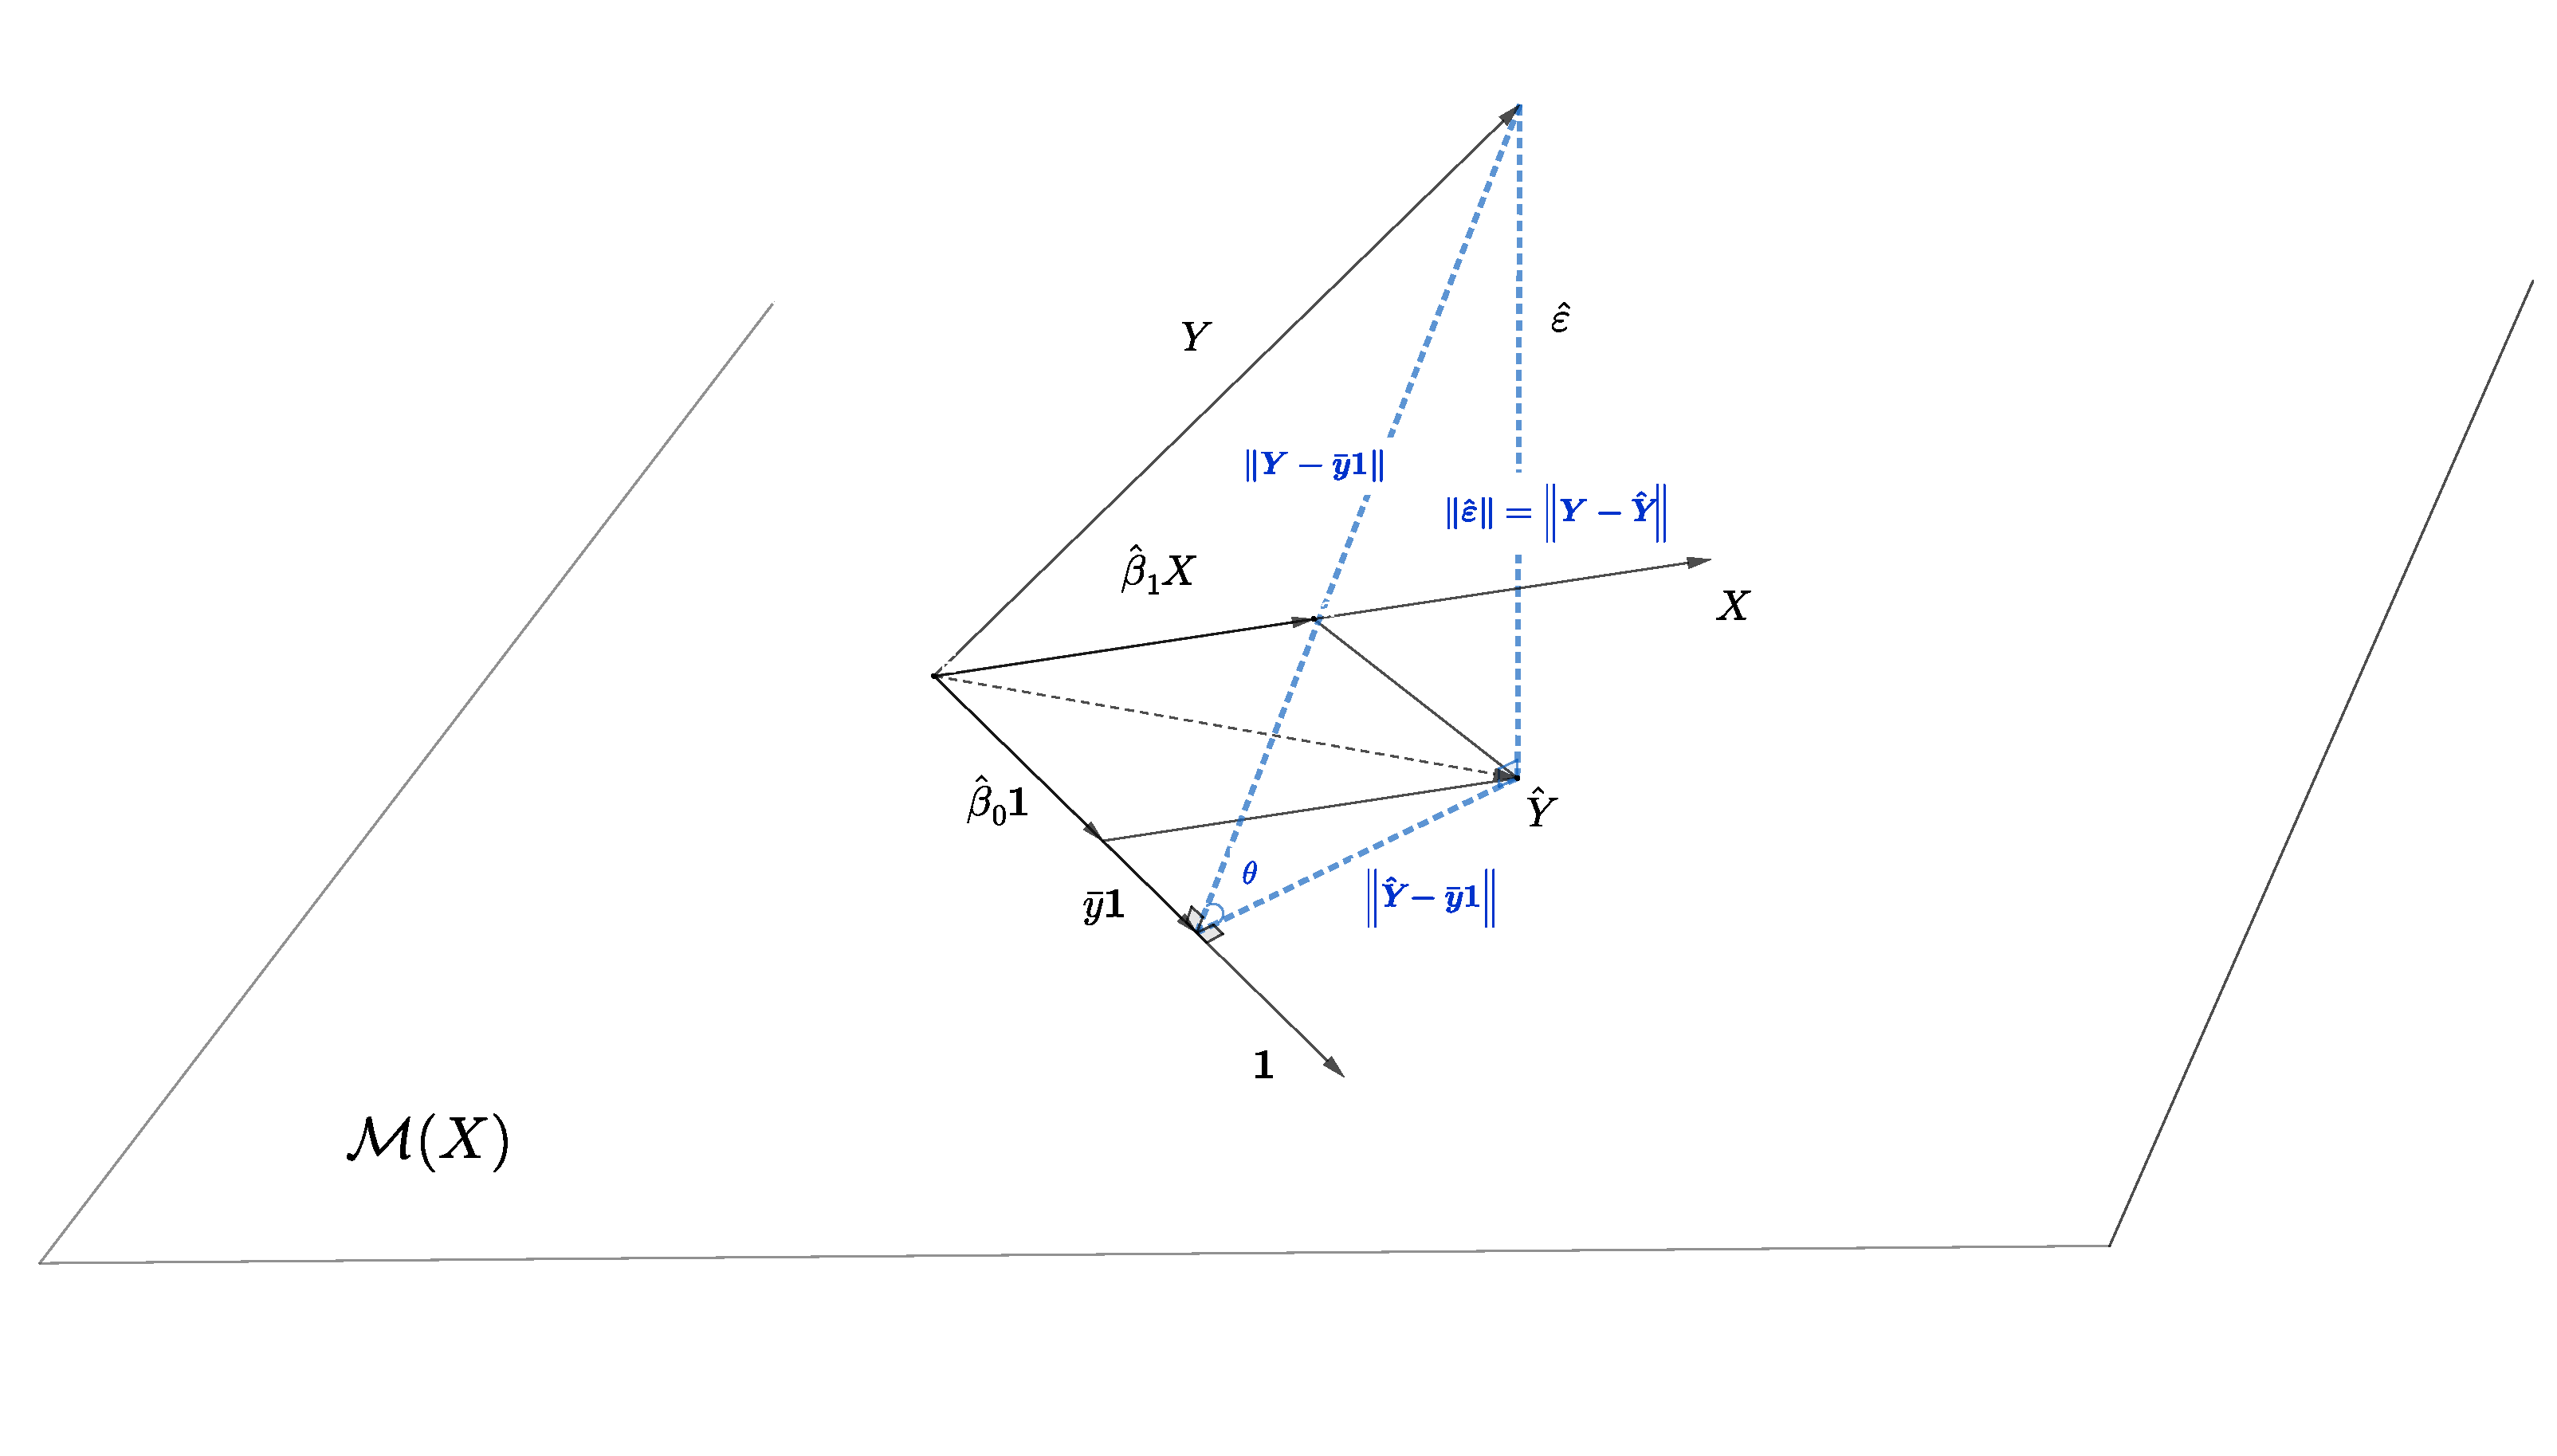
\includegraphics[width=0.8\linewidth]{images/lab5/reg_int_geom5} \end{center}

Observăm că, în general, vectorii \(\{\mathbf{1}, X\}\) nu formează o
bază ortogonală în \(\mathcal{M}(X)\) (cu excepția cazului în care
\(\langle \mathbf{1}, X\rangle = n\bar x = 0\)) prin urmare
\(\hat\beta_0\mathbf{1}\) nu este proiecția ortogonală a lui \(Y\) pe
\(\mathbf{1}\) (aceasta este
\(\frac{\langle Y, \mathbf{1}\rangle}{\lVert \mathbf{1}\rVert^2}\mathbf{1} = \bar y\mathbf{1}\))
iar \(\hat\beta_1 X\) nu este proiecția ortogonală a lui \(Y\) pe \(X\)
(aceasta fiind \(\frac{\langle Y, X\rangle}{\lVert X\rVert^2}X\)).

Fie
\(\hat\varepsilon = Y - \hat Y = (\hat\varepsilon_1, \hat\varepsilon_2, \ldots, \hat\varepsilon_n)^\intercal\)
vectorul valorilor reziduale. Aplicând Teorema lui Pitagora (în
triunghiul albastru) rezultă (descompunerea ANOVA pentru regresie) că

\begin{align*}
  \left\lVert Y - \bar y \mathbf{1}\right\rVert^2 &= \left\lVert \hat Y - \bar y \mathbf{1}\right\rVert^2 + \left\lVert \underbrace{\hat\varepsilon}_{Y - \hat Y}\right\rVert^2\\
  \sum_{i = 1}^{n}(y_i - \bar y)^2 &= \sum_{i = 1}^{n}(\hat y_i - \bar y)^2 + \sum_{i = 1}^{n}(\underbrace{\hat\varepsilon_i}_{y_i - \hat y_i})^2\\
  SS_T &= SS_{reg} + RSS
\end{align*}

Din definiția coeficientului de determinare \(R^2\) avem că

\[
R^2 = \frac{SS_{reg}}{SS_T} = \frac{\left\lVert \hat Y - \bar y \mathbf{1}\right\rVert^2}{\left\lVert Y - \bar y \mathbf{1}\right\rVert^2} = 1 - \frac{\left\lVert \hat \varepsilon\right\rVert^2}{\left\lVert Y - \bar y \mathbf{1}\right\rVert^2}
\]

și conform figurii de mai sus \(R^2 = \cos^2(\theta)\). Prin urmare dacă
\(R^2 = 1\), atunci \(\theta = 0\) și \(Y\in\mathcal{M}(X)\), deci
\(y_i = \beta_0 + \beta_1 x_i\), \(i\in\{1,2,\ldots,n\}\) (punctele
eșantionului sunt perfect aliniate) iar dacă \(R^2 = 0\), deducem că
\(\sum_{i = 1}^{n}(\hat y_i - \bar y)^2 = 0\), deci
\(\hat y_i = \bar y\) (modelul liniar nu este adaptat în acest caz, nu
putem explica mai bine decât media).

\subsection{Exercițiul 1}\label{exercitiul-1}

\begin{rmdexercise}
Arătați că estimatorii obținuți prin metoda celor mai mici pătrate,
\(\hat\beta_0\) și \(\hat\beta_1\), sunt estimatori nedeplasați.
\end{rmdexercise}

Coeficienții \(\hat\beta_0\) și \(\hat\beta_1\) obținuți prin metoda
celor mai mici pătrate sunt dați de
\(\hat\beta_0 = \bar y - \hat\beta_1 \bar x\) și
\(\hat\beta_1 = \frac{\sum_{i = 1}^{n}(x_i - \bar x)(y_i - \bar y)}{\sum_{i = 1}^{n}(x_i - \bar x)^2}\)
(aceștia sunt variabile aleatoare deoarece sunt funcții de \(Y_i\) care
sunt variabile aleatoare). Înlocuind în expresia lui \(\hat\beta_1\) pe
\(y_i\) cu \(\beta_0+\beta_1 x_i + \varepsilon_i\) avem

\begin{align*}
\hat\beta_1 &= \frac{\sum_{i = 1}^{n}(x_i - \bar x)(y_i - \bar y)}{\sum_{i = 1}^{n}(x_i - \bar x)^2} = \frac{\sum_{i = 1}^{n}(x_i - \bar x)y_i}{\sum_{i = 1}^{n}(x_i - \bar x)^2} = \frac{\sum_{i = 1}^{n}(x_i - \bar x)(\beta_0+\beta_1 x_i + \varepsilon_i)}{\sum_{i = 1}^{n}(x_i - \bar x)^2}\\
  &= \frac{\beta_0\overbrace{\sum_{i = 1}^{n}(x_i - \bar x)}^{ = 0} + \beta_1 \sum_{i = 1}^{n}(x_i - \bar x)x_i + \sum_{i = 1}^{n}(x_i - \bar x)\varepsilon_i}{\sum_{i = 1}^{n}(x_i - \bar x)^2} = \frac{\beta_1 \sum_{i = 1}^{n}(x_i - \bar x)^2 + \sum_{i = 1}^{n}(x_i - \bar x)\varepsilon_i}{\sum_{i = 1}^{n}(x_i - \bar x)^2}\\
  &= \beta_1 + \frac{\sum_{i = 1}^{n}(x_i - \bar x)\varepsilon_i}{\sum_{i = 1}^{n}(x_i - \bar x)^2}.
\end{align*}

Conform ipotezei modelului de regresie liniară simplă,
\(\mathbb{E}[\varepsilon_i] = 0\), prin urmare
\(\mathbb{E}[\hat\beta_1] = \beta_1\) ceea ce arată că \(\hat\beta_1\)
este un estimator nedeplasat pentru \(\beta_1\).

În mod similar,

\[
\mathbb{E}[\hat\beta_0] = \mathbb{E}[\bar y] - \bar x\mathbb{E}[\hat\beta_1] = \beta_0 + \bar x\beta_1 - \bar x\beta_1 = \beta_0
\] ceea ce arată că \(\hat\beta_0\) este un estimator nedeplasat pentru
\(\beta_0\).

\begin{rmdexercise}
Calculați matricea de varianță-covarianță a estimatorilor
\(\hat\beta_0\) și \(\hat\beta_1\).
\end{rmdexercise}

Notăm cu
\(W = \begin{pmatrix}Var(\hat \beta_0) & Cov(\hat \beta_0, \hat \beta_1)\\ Cov(\hat \beta_0, \hat \beta_1) & Var(\hat \beta_1)\end{pmatrix}\)
matricea de varianță-covarianță a estimatorilor \(\hat\beta_0\) și
\(\hat\beta_1\).

Avem, folosind expresia lui \(\hat\beta_1\) determinată la punctul
anterior și homoscedasticitatea și necorelarea erorilor
\(Cov(\varepsilon_i, \varepsilon_j) = \delta_{ij}\sigma^2\), că

\begin{align*}
  Var(\hat \beta_1) &= Var\left(\beta_1 + \frac{\sum_{i = 1}^{n}(x_i - \bar x)\varepsilon_i}{\sum_{i = 1}^{n}(x_i - \bar x)^2}\right) = Var\left(\frac{\sum_{i = 1}^{n}(x_i - \bar x)\varepsilon_i}{\sum_{i = 1}^{n}(x_i - \bar x)^2}\right)\\
  &= \frac{Var\left(\sum_{i = 1}^{n}(x_i - \bar x)\varepsilon_i\right)}{\left[\sum_{i = 1}^{n}(x_i - \bar x)^2\right]^2} = \frac{\sum_{i,j}(x_i - \bar x)(x_j - \bar x)Cov(\varepsilon_i, \varepsilon_j)}{\left[\sum_{i = 1}^{n}(x_i - \bar x)^2\right]^2}\\
  &= \frac{\sum_{i = 1}^{n}(x_i - \bar x)^2\sigma^2}{\left[\sum_{i = 1}^{n}(x_i - \bar x)^2\right]^2} = \frac{\sigma^2}{\sum_{i = 1}^{n}(x_i - \bar x)^2}.
\end{align*}

Din expresia \(Var(\hat \beta_1)\) observăm că dacă \(\sigma^2\) este
mică (cu alte cuvinte \(y_i\) sunt aproape de dreapta de regresie)
atunci estimarea este mai precisă. De asemenea, se constată că pe măsură
ce valorile \(x_i\) sunt mai dispersate în jurul valorii medii
\(\bar x\) estimarea coeficientului \(\hat \beta_1\) este mai precisă
(\(Var(\hat \beta_1)\) este mai mică). Acest fenomen se poate observa și
în figura de mai jos în care am generat \(100\) de valori aleatoare
\(X\) și \(100\) de valori pentru \(Y\) după modelul

\[
  y = 1 + 2 x + \varepsilon
\] cu \(\varepsilon\sim \mathcal{N}(0, \sigma^2)\). Dreapta roșie
descrie adevărata relație \(f(x) = 1 + 2x\) în populație iar dreapta
albastră reprezintă dreapta de regresie calculată cu ajutorul metodei
celor mai mici pătrate (OLS). Dreptele albastru deschis au fost generate
tot cu ajutorul metodei celor mai mici pătrate atunci când variem
\(\sigma^2\) (în figura din stânga) și respectiv pe \(x_i\) în jurul lui
\(\bar x\) (în figura din dreapta).

\begin{center}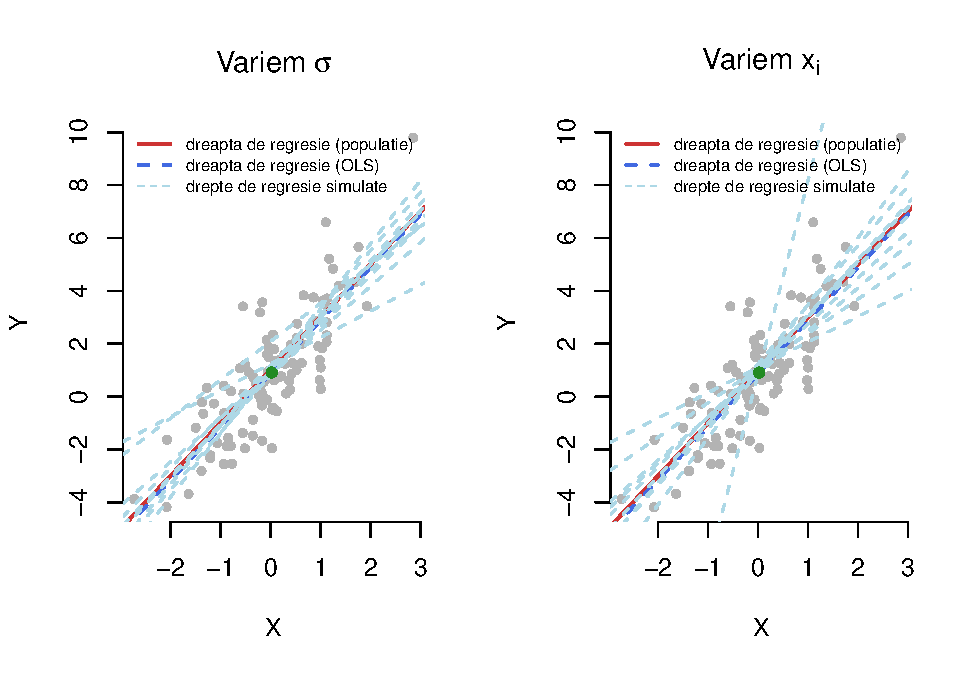
\includegraphics[width=0.7\linewidth]{Sem_2_files/figure-latex/unnamed-chunk-5-1} \end{center}

Pentru a determina \(Var(\hat \beta_0)\), vom folosi relația
\(\hat \beta_0 = \bar y - \hat \beta_1 \bar x\) ceea ce conduce la

\begin{align*}
Var(\hat \beta_0) &= Var(\bar y - \hat \beta_1 \bar x) = Var(\bar y) - 2Cov(\bar y, \hat \beta_1 \bar x) + Var(\hat \beta_1 \bar x)\\
&= Var\left(\frac{1}{n}\sum_{i = 1}^{n}y_i\right) - 2\bar x Cov(\bar y, \hat \beta_1) + \bar x^2 Var(\hat \beta_1)\\
&= \frac{\sigma^2}{n} + \bar x^2 \frac{\sigma^2}{\sum_{i = 1}^{n}(x_i - \bar x)^2} - 2\bar x Cov(\bar y, \hat \beta_1).
\end{align*}

Pentru \(Cov(\bar y, \hat \beta_1)\) avem (ținând cont de faptul că
\(\beta_0\), \(\beta_1\) și \(x_i\) sunt constante)

\begin{align*}
Cov(\bar y, \hat \beta_1) &= Cov\left(\frac{1}{n}\sum_{i = 1}^{n}y_i, \beta_1 + \frac{\sum_{j = 1}^{n}(x_j - \bar x)\varepsilon_j}{\sum_{j = 1}^{n}(x_j - \bar x)^2} \right) = \frac{1}{n}\sum_{i = 1}^{n}Cov\left(\beta_0 + \beta_1 x_i + \varepsilon_i, \beta_1 + \frac{\sum_{j = 1}^{n}(x_j - \bar x)\varepsilon_j}{\sum_{j = 1}^{n}(x_j - \bar x)^2}\right)\\
&= \frac{1}{n}\sum_{i = 1}^{n}Cov\left(\varepsilon_i, \frac{\sum_{j = 1}^{n}(x_j - \bar x)\varepsilon_j}{\sum_{j = 1}^{n}(x_j - \bar x)^2}\right) = \frac{1}{n}\sum_{i = 1}^{n}\frac{1}{\sum_{j = 1}^{n}(x_j - \bar x)^2}Cov\left(\varepsilon_i, \sum_{j = 1}^{n}(x_j - \bar x)\varepsilon_j\right)\\
&= \frac{1}{\sum_{j = 1}^{n}(x_j - \bar x)^2}\sum_{i = 1}^{n}\frac{1}{n}\sum_{j = 1}^{n}(x_j - \bar x)Cov(\varepsilon_i, \varepsilon_i=j) = \frac{1}{\sum_{j = 1}^{n}(x_j - \bar x)^2}\sum_{i = 1}^{n}\frac{1}{n}\sum_{j = 1}^{n}(x_j - \bar x)\delta_{ij}\sigma^2\\
&= \frac{\sigma^2}{\sum_{j = 1}^{n}(x_j - \bar x)^2}\frac{1}{n}\underbrace{\sum_{i = 1}^{n}(x_i - \bar x)}_{=0} = 0
\end{align*}

prin urmare

\[
Var(\hat \beta_0) = \frac{\sigma^2}{n} + \bar x^2 \frac{\sigma^2}{\sum_{i = 1}^{n}(x_i - \bar x)^2} = \frac{\sigma^2\sum_{i = 1}^{n}x_i^2}{n\sum_{i = 1}^{n}(x_i - \bar x)^2}.
\]

Calculul covarianței dintre \(\hat \beta_0\) și \(\hat \beta_1\) rezultă
aplicând relațiile de mai sus

\[
Cov(\hat \beta_0, \hat \beta_1) = Cov(\bar y - \hat \beta_1\bar x, \hat \beta_1) = Cov(\bar y, \hat \beta_1) - \bar x Var(\hat \beta_1) = -\frac{\sigma^2 \bar x}{\sum_{i = 1}^{n}(x_i - \bar x)^2}.
\]

Observăm că \(Cov(\hat \beta_0, \hat \beta_1)\leq 0\) iar intuitiv, cum
dreapta de regresie (bazată pe estimatorii obținuți prin metoda celor
mai mici pătrate) \(\bar y = \hat\beta_0 + \hat\beta_1 \bar x\) trece
prin centrul de greutate al datelor \((\bar x, \bar y)\), dacă
presupunem \(\bar x > 0\) remarcăm că atunci când creștem panta (creștem
\(\hat\beta_1\)) ordonata la origine scade (scade \(\hat\beta_0\)) și
reciproc.

Matricea de varianță-covarianță a estimatorilor \(\hat\beta_0\) și
\(\hat\beta_1\) devine

\[
W = \begin{pmatrix}Var(\hat \beta_0) & Cov(\hat \beta_0, \hat \beta_1)\\ Cov(\hat \beta_0, \hat \beta_1) & Var(\hat \beta_1)\end{pmatrix} = \begin{pmatrix}\frac{\sigma^2\sum_{i = 1}^{n}x_i^2}{n\sum_{i = 1}^{n}(x_i - \bar x)^2} & -\frac{\sigma^2 \bar x}{\sum_{i = 1}^{n}(x_i - \bar x)^2}\\ -\frac{\sigma^2 \bar x}{\sum_{i = 1}^{n}(x_i - \bar x)^2} & \frac{\sigma^2}{\sum_{i = 1}^{n}(x_i - \bar x)^2}\end{pmatrix}.
\]

\begin{rmdexercise}
Arătați că în cadrul modelului de regresie liniară simplă, suma
valorilor reziduale este nulă.
\end{rmdexercise}

Observăm, folosind definiția \(\hat\varepsilon_i = y_i - \hat y_i\), că

\begin{align*}
  \sum_{i = 1}^{n}\hat\varepsilon_i &= \sum_{i = 1}^{n}(y_i - \hat y_i) = \sum_{i = 1}^{n}(y_i - \hat \beta_0 - x_i\hat\beta_1)\\
    &= \sum_{i = 1}^{n}\left[y_i - \underbrace{(\bar y - \bar x\hat\beta_1)}_{= \hat \beta_0} - x_i\hat\beta_1\right] = \sum_{i = 1}^{n}(y_i - \bar y) -\hat\beta_1 \sum_{i = 1}^{n}(x_i - \bar x) = 0
\end{align*}

\begin{rmdexercise}
Arătați că în modelul de regresie liniară simplă statistica
\(\hat\sigma^2 = \frac{1}{n-2}\sum_{i = 1}^{n}\hat\varepsilon_i^2\) este
un estimator nedeplasat pentru \(\sigma^2\).
\end{rmdexercise}

Ținând cont de faptul că \(\hat\beta_0 = \bar y - \hat\beta_1 \bar x\)
și \(\bar y = \beta_0 + \beta_1 \bar x + \bar \varepsilon\) (prin
însumarea după \(i\) a relațiilor
\(y_i = \beta_0 + \beta_1 x_i +\varepsilon_i\)) găsim că

\begin{align*}
\hat\varepsilon_i &= y_i - \hat y_i = (\beta_0 + \beta_1 x_i +\varepsilon_i) - (\hat\beta_0 + \hat\beta_1 x_i) \\
  &= (\underbrace{\bar y - \beta_1 \bar x - \bar \varepsilon}_{=\beta_0} + \beta_1 x_i +\varepsilon_i) - (\bar y - \hat\beta_1 \bar x + \hat\beta_1 x_i)\\
  &= (\beta_1 - \hat\beta_1)(x_i - \bar x) + (\varepsilon_i - \bar\varepsilon)
\end{align*}

și prin dezvoltarea binomului și utilizând relația
\(\hat\beta_1 = \beta_1 + \frac{\sum_{i = 1}^{n}(x_i - \bar x)\varepsilon_i}{\sum_{i = 1}^{n}(x_i - \bar x)^2}\)
găsim

\begin{align*}
  \sum_{i = 1}^{n}\hat\varepsilon_i^2 &= (\beta_1 - \hat\beta_1)^2\sum_{i = 1}^{n}(x_i - \bar x) + \sum_{i = 1}^{n}(\varepsilon_i - \bar\varepsilon)^2 + 2(\beta_1 - \hat\beta_1)\sum_{i = 1}^{n}(x_i - \bar x)(\varepsilon_i - \bar\varepsilon)\\
    &= (\beta_1 - \hat\beta_1)^2\sum_{i = 1}^{n}(x_i - \bar x) + \sum_{i = 1}^{n}(\varepsilon_i - \bar\varepsilon)^2 + 2(\beta_1 - \hat\beta_1)\sum_{i = 1}^{n}(x_i - \bar x)\varepsilon_i - 2(\beta_1 - \hat\beta_1)\bar\varepsilon\sum_{i = 1}^{n}(x_i - \bar x)\\
    &= (\beta_1 - \hat\beta_1)^2\sum_{i = 1}^{n}(x_i - \bar x) + \sum_{i = 1}^{n}(\varepsilon_i - \bar\varepsilon)^2 - 2(\beta_1 - \hat\beta_1)^2\sum_{i = 1}^{n}(x_i - \bar x)^2\\
    &=\sum_{i = 1}^{n}(\varepsilon_i - \bar\varepsilon)^2 - (\beta_1 - \hat\beta_1)^2\sum_{i = 1}^{n}(x_i - \bar x)^2.
\end{align*}

Luând media găsim că

\[
\mathbb{E}\left(\sum_{i = 1}^{n}\hat\varepsilon_i^2\right) = \mathbb{E}\left(\sum_{i = 1}^{n}(\varepsilon_i - \bar\varepsilon)^2\right) - \sum_{i = 1}^{n}(x_i - \bar x)^2 Var(\hat\beta_1) = (n-1)\sigma^2 - \sigma^2 = (n-1)\sigma^2
\]

unde am folosit că
\(\mathbb{E}\left(\frac{1}{n-1}\sum_{i = 1}^{n}(\varepsilon_i - \bar\varepsilon)^2\right) = \sigma^2\)
(deoarece \(Var(\varepsilon_i) = \sigma^2\)).

Concluzionăm că
\(\hat\sigma^2 = \frac{1}{n-2}\sum_{i = 1}^{n}\hat\varepsilon_i^2\) este
un estimator nedeplasat pentru \(\sigma^2\).

\begin{rmdexercise}
Fie \(x_{n+1}\) o nouă valoare pentru variabila \(X\) și ne propunem să
prezicem valoarea \(y_{n+1}\) conform modelului

\[
  y_{n+1} = \beta_0 + \beta_1 x_{n+1} + \varepsilon_{n+1}
\]

cu \(\mathbb{E}[\varepsilon_{n+1}] = 0\),
\(Var(\varepsilon_{n+1}) = \sigma^2\) și
\(Cov(\varepsilon_{n+1}, \varepsilon_i)=0\) pentru \(i = 1,\ldots,n\).

Arătați că varianța răspunsului mediu prezis este

\[
  Var(\hat y_{n+1}) = \sigma^2\left[\frac{1}{n} + \frac{(x_{n+1} - \bar x)^2}{\sum_{i=1}^{n}(x_i - \bar x)^2}\right]
\]

iar varianța erorii de predicție \(\hat\varepsilon_{n+1}\) satisface
\(\mathbb{E}[\hat\varepsilon_{n+1}] = 0\) și

\[
  Var(\hat\varepsilon_{n+1}) = \sigma^2\left[1 + \frac{1}{n} + \frac{(x_{n+1} - \bar x)^2}{\sum_{i=1}^{n}(x_i - \bar x)^2}\right].
\]
\end{rmdexercise}

Cum \(\hat y_{n+1} = \hat\beta_0 + \hat\beta_1 x_{n+1}\) avem

\begin{align*}
  Var(\hat y_{n+1}) &= Var(\hat\beta_0 + \hat\beta_1 x_{n+1}) = Var(\hat\beta_0) + 2Cov(\hat\beta_0, \hat\beta_1) + x_{n+1}^2Var(\hat\beta_1)\\
  &= \frac{\sigma^2\sum_{i = 1}^{n}x_i^2}{n\sum_{i = 1}^{n}(x_i - \bar x)^2} - 2\frac{\sigma^2 \bar x}{\sum_{i = 1}^{n}(x_i - \bar x)^2} + \frac{\sigma^2x_{n+1}^2}{\sum_{i = 1}^{n}(x_i - \bar x)^2}\\
  &= \frac{\sigma^2}{\sum_{i = 1}^{n}(x_i - \bar x)^2}\left[\frac{1}{n}\sum_{i = 1}^{n}x_i^2 - 2x_{n+1}\bar x + x_{n+1}^2\right]\\
  &= \frac{\sigma^2}{\sum_{i = 1}^{n}(x_i - \bar x)^2}\left[\frac{1}{n}\sum_{i = 1}^{n}(x_i -\bar x)^2 + \bar x^2 - 2x_{n+1}\bar x + x_{n+1}^2\right]\\
  &= \sigma^2\left[\frac{1}{n} + \frac{(x_{n+1} - \bar x)^2}{\sum_{i=1}^{n}(x_i - \bar x)^2}\right].
\end{align*}

Constatăm că atunci când \(x_{n+1}\) este departe de valoarea medie
\(\bar x\) răspunsul mediu are o variabilitate mai mare.

Pentru a obține varianța erorii de predicție
\(\hat\varepsilon_{n+1} = y_{n+1} - \hat y_{n+1}\) să observăm că
\(y_{n+1}\) depinde doar de \(\varepsilon_{n+1}\) pe când
\(\hat y_{n+1}\) depinde de \(\varepsilon_i\), \(i\in\{1,2,\ldots,n\}\).
Din necorelarea erorilor deducem că

\[
  Var(\hat\varepsilon_{n+1}) = Var(y_{n+1} - \hat y_{n+1}) = Var(y_{n+1}) + Var(\hat y_{n+1}) = \sigma^2\left[1 + \frac{1}{n} + \frac{(x_{n+1} - \bar x)^2}{\sum_{i=1}^{n}(x_i - \bar x)^2}\right].
\]

\subsection{\texorpdfstring{Exercițiul 2: Coeficientul de determinare
\(R^2\) și coeficientul de
corelație}{Exercițiul 2: Coeficientul de determinare R\^{}2 și coeficientul de corelație}}\label{exercitiul-2-coeficientul-de-determinare-r2-si-coeficientul-de-corelatie}

\begin{rmdexercise}
Arătați că

\[
  R^2 = r_{xy}^2 = r_{y\hat y}^2
\]

unde \(r_{xy}\) este coeficientul de corelație empiric dintre \(x\) și
\(y\).
\end{rmdexercise}

Din definiția coeficientului de determinare și folosind coeficienții
\(\hat\beta_0 = \bar y - \hat\beta_1 \bar x\) și
\(\hat\beta_1 = \frac{\sum_{i = 1}^{n}(x_i - \bar x)(y_i - \bar y)}{\sum_{i = 1}^{n}(x_i - \bar x)^2}\)
obținuți prin metoda celor mai mici pătrate avem

\begin{align*}
R^2 &= \frac{\left\lVert \hat Y - \bar y \mathbf{1}\right\rVert^2}{\left\lVert Y - \bar y \mathbf{1}\right\rVert^2} = \frac{\sum_{i = 1}^{n}(\hat\beta_0 + \hat\beta_1 x_i - \bar y)^2}{\sum_{i = 1}^{n}(y_i - \bar y)^2} = \frac{\sum_{i = 1}^{n}(\bar y - \hat\beta_1 \bar x + \hat\beta_1\bar x - \bar y)^2}{\sum_{i = 1}^{n}(y_i - \bar y)^2}\\
  &= \frac{\hat\beta_1^2\sum_{i = 1}^{n}(x_i - \bar x)^2}{\sum_{i = 1}^{n}(y_i - \bar y)^2} = \left(\frac{\sum_{i = 1}^{n}(x_i - \bar x)(y_i - \bar y)}{\sum_{i = 1}^{n}(x_i - \bar x)^2}\right)^2\frac{\sum_{i = 1}^{n}(x_i - \bar x)^2}{\sum_{i = 1}^{n}(y_i - \bar y)^2}\\
  & = \frac{\left[\sum_{i = 1}^{n}(x_i - \bar x)(y_i - \bar y)\right]^2}{\sum_{i = 1}^{n}(x_i - \bar x)^2\sum_{i = 1}^{n}(y_i - \bar y)^2} = r_{xy}^2.
\end{align*}

Pentru a verifica a doua parte, \(R^2 = r_{y\hat y}^2\), să observăm că

\[
r_{y\hat y}^2 = \frac{\left[\sum_{i = 1}^{n}(\hat y_i - \bar{\hat y})(y_i - \bar y)\right]^2}{\sum_{i = 1}^{n}(\hat y_i - \bar{\hat y})^2\sum_{i = 1}^{n}(y_i - \bar y)^2}
\]

iar
\(\bar{\hat y} = \frac{\sum_{i = 1}^{n}\hat y_i}{n} = \hat \beta_0 + \hat\beta_1 \bar x = \bar y\),
prin urmare

\[
r_{y\hat y}^2 = \frac{\left[\sum_{i = 1}^{n}(\hat y_i - \bar{y})(y_i - \bar y)\right]^2}{\sum_{i = 1}^{n}(\hat y_i - \bar{y})^2\sum_{i = 1}^{n}(y_i - \bar y)^2}.
\]

De asemenea

\begin{align*}
\sum_{i = 1}^{n}(\hat y_i - \bar{y})(y_i - \bar y) &= \sum_{i = 1}^{n}(\hat y_i - \bar{y})(y_i - \hat y_i + \hat y_i - \bar y) \\
 &= \sum_{i = 1}^{n}(\hat y_i - \bar{y})(y_i - \hat y_i) + \sum_{i = 1}^{n}(\hat y_i - \bar{y})^2
\end{align*}

și cum

\begin{align*}
\sum_{i = 1}^{n}(\hat y_i - \bar{y})(y_i - \hat y_i) &= \sum_{i = 1}^{n}(\hat \beta_0 + \hat\beta_1 x_i - \bar{y})(y_i - \hat \beta_0 - \hat\beta_1 x_i) \\
  &= \sum_{i = 1}^{n}(\bar y - \hat\beta_1 \bar x + \hat\beta_1 x_i - \bar{y})[(y_i - \bar y ) - \hat\beta_1 (x_i - \bar x)]\\
  &= \hat\beta_1 \sum_{i = 1}^{n}(x_i - \bar x)(y_i - \bar y) - \hat\beta_1^2 \sum_{i = 1}^{n}(x_i - \bar x)^2 \\
  &= \underbrace{\frac{S_{xy}}{S_{xx}}}_{\hat\beta_1}S_{xy} - \frac{S_{xy}^2}{S_{xx}^2}S_{xx} = 0
\end{align*}

deducem că
\(r_{y\hat y}^2 = \frac{\sum_{i = 1}^{n}(\hat y_i - \bar{y})^2}{\sum_{i = 1}^{n}(y_i - \bar y)^2} = R^2\).

\bibliography{references/InstStatFin2018ref.bib}


\end{document}
